\documentclass[12pt, twoside]{report}
\usepackage[a4paper,bindingoffset=0.2in,%
            left=0.8in,right=0.8in,top=1.2in,bottom=1.2in,%
			]{geometry}
\usepackage{graphicx}
\usepackage{subfig}
\usepackage{fancyhdr}
\fancyhf{}
\renewcommand{\headrulewidth}{0pt}
\fancyhead[RO,LE]{\thepage}
\pagestyle{fancy}

\begin{document}

\chapter{Chapter 2}
 
\chapter{\huge Background and Literature Review}
The importance of facial expression in social interaction and social intelligence is widely
recognized. Facial expression analysis has been an active research topic since 19th century.
The first automatic facial expression recognition system was introduced in 1978 by Suwa
et al. [83]. This system attempts to analyze facial expressions by tracking the motion of
20 identified spots on an image sequence. Since then, a lot of work has been done in this
domain. Various computer systems have been made to help us understand and use this
natural form of human communication.\par
This chapter reviews the state of the art of what has been done in processing and
understanding facial expression. When building an FER system, these main issues must
be considered: face detection and alignment, image normalization, feature extraction, and
classification. Most of the current work in FER is based on methods that implement these
steps sequentially and independently. Before exploring what has been done in literature for
implementing these steps, we will briefly describe the problem space for facial expression
analysis.
\section{Problem Space for Facial Expression Analysis}
\subsection{Level of Description}
In general there are two types of method to describe facial expression.
\newpage
\subsubsection{Facial Action Coding System}
\par 
The facial action coding system [24] is a human-observer-based system widely used in
psychology to describe subtle changes in facial features. FACS consists of 44 action units
which are related to contraction of a specific set of facial muscles (Fig.2.1). Some of the
action units are shown in Fig.2.2. Conventional, FACS code is manually labeled by trained
observers while viewing videotaped facial behavior in slow motion. In recent years, some
attempts have been made to do this automatically [69]. The advantage of FACS is its ability
to capture the subtlety of facial expression, however FACS itself is purely descriptive and
includes no inferential labels. That means in order to get the emotion estimation, the FACS
code needs to be converted into the Emotional Facial Action System (EMFACS [28]) or
similar systems.\\

\begin{figure}[h]%
	\begin{minipage}[b]{.5\textwidth}
    \centering
    \subfloat{{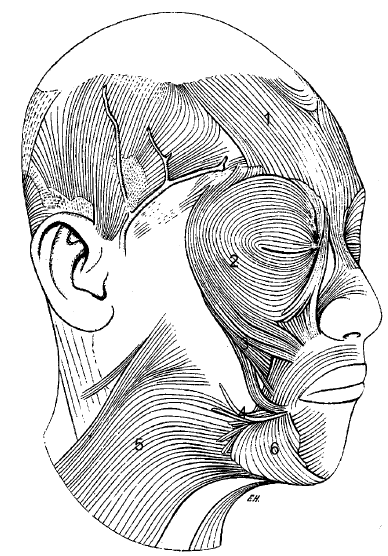
\includegraphics[width=5cm]{img/Page-2-Image-1.png} }}%
\caption{Muscles of facial expression. 1,
frontalis; 2, orbicularis oculi; 3, zygomaticus
major; 4, risorius; 5, platysma; 6, depressor
anguli oris [33]}
\end{minipage}
\hfill
\begin{minipage}[b]{.5\textwidth}
    \subfloat{{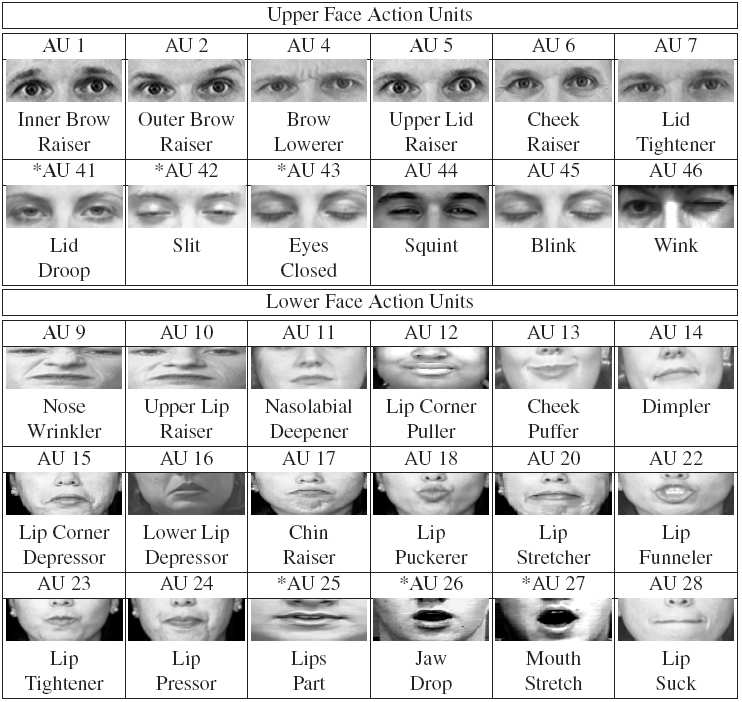
\includegraphics[width=7cm]{img/Page-2-Image-2.png} }}%
\centering
\caption{FACS action units [35]}
\end{minipage}
	\label{fig:example}%
\end{figure}
\end{document}